\newpage 
\section{Numerical Results} \label{s4}
With the theoretical background described in the previous sections, this section demonstrates the capabilities of the proposed framework in addressing multi-physics problems using several test cases, ranging from two-dimensional pin-cell problems to whole-core problems. Most of the problems presented in this thesis use material compositions and geometry adapted from the Virtual Environment for Reactor Applications (VERA) core physics benchmark \cite{godfrey}. Additionally, ENDF/B-VII.1 was used for the MCS cross section library.

This section is divided into three subsections. Subsection \ref{sec41} provides the solutions for MC coupled multi-physics with spatially continuous material properties. While the solutions for thermal expansion are presented in subsection \ref{sec42}. Lastly, subsection \ref{sec43} presents the solutions for assembly and whole-core problems using both spatially continuous material and thermal expansion methods.

\subsection{Spatially Continuous Material Properties} \label{sec41}

This subsection presents and discusses the solutions for MC coupled multi-physics simulations with spatially continuous material properties. For multi-physics feedback in all problem cases in this subsection, unless specified otherwise, radial heat conduction calculations within the fuel pellet were conducted using 10 radial rings, while a single mesh was employed for the gap and cladding regions. The resulting radial fuel temperature distribution was then averaged based on the number of radial cells used in the neutronic calculations.

In the conventional or cell-based approach, the problem geometry was discretized into several cells, with material properties such as temperature and density being uniform within each cell. This discretization was necessary to capture material property variations across the problem geometry. In contrast, in the FET-based cases, explicit problem geometry discretization was unnecessary. Instead, the power and Xenon absorption rates distributions were reconstructed using 100 axial and 10 radial equidistant meshes for each pin during each TH update and equilibrium Xenon feedback, respectively.

For tally reconstruction, seventh-order Legendre polynomials and ninth-order Zernike polynomials were used in the axial and radial directions, respectively.

\subsubsection{Two-dimensional Pin-cell Problem}

This two-dimensional pin-cell problem, based on the work of Choi and Joo \cite{nchoi_2020}, is designed to evaluate the temperature distribution within a fuel pellet and its influence on spatial self-shielding. The case involves a two-dimensional pin-cell multi-physics model, utilizing UO$_2$ fuel enriched to 2.1 wt.\% and a linear power density of 175 W/cm. To maintain a constant axial profile, the coolant flow rate is assumed to be infinite. The coolant bulk temperature is fixed at 600K, with no boron dilution in the coolant.

Three cases are presented in this problem, as outlined in Table \ref{tab2}. Each case varies in the number of radial cells used for neutronic calculations. Cases A1, A2, and A3 are cell-based, with discretization into 1, 5, and 20 equally spaced radial cells, respectively. The results from these cases are compared to those obtained from the FET case, which utilizes continuous fuel temperature. It is important to note that all simulations used $5\times10^4$ particles per cycle, over a total of 30,000 cycles, with 27,500 cycles designated as active.
\begin{table}
    \centering
    \caption{Two-dimensional pin-cell problem infinite multiplication factors.}
    \label{tab2} 
    % \begin{adjustbox}{width=0.6\textwidth} % Adjust your table to the text width
    \begin{tabular}{| c | c | c | }
    \hline 
     Cases & \# radial discretization & $k_{inf}$ \\
     \hline
     A1     & 1   & $1.22203\pm0.00002$      \\ \hline
     A2     & 5   & $1.22250\pm0.00002$      \\ \hline
     A3     & 20  & $1.22259\pm0.00002$      \\ \hline
     FET    & N/A & $1.22261\pm0.00002$      \\ \hline
     Extrapolation    & N/A & $1.22262$      \\ \hline
    \end{tabular}
    % \end{adjustbox}
\end{table}

The continuous fuel temperature from the FET case is compared to the piecewise fuel temperature from the other cases in Figure \ref{fig_41}. As shown, the continuous temperature from the FET case closely aligns with the piecewise fuel temperature as the mesh refinement increases. For a direct comparison, radial mesh tallies for absorption and fission rates across 20 meshes were conducted during the simulation, with the results displayed in Figure \ref{fig_42}. The figure demonstrates that the proposed framework yields increasingly accurate solutions as the mesh size decreases, which confirms the correct implementation of the framework into the MCS code. The differences in absorption rates between cases A2 and A3 and the FET case are less than 1.0\%, while the A1 case overestimates the self-shielding absorption at the fuel pellet's periphery by up to 2.6\%, due to the higher peripheral fuel temperature in the A1 case. In contrast, the fission rate remains relatively uniform with no significant differences, as thermal neutrons that responsible for fission are less affected by self-shielding. The combination of higher resonance absorption at the fuel pellet periphery and a relatively flat fission rate distribution results in a lower infinite multiplication factor ($k_{inf}$), as observed in the A1 case (see Table \ref{tab2}).

\begin{figure}
      \centering
      \includegraphics[width=0.5\textwidth]{figs/pin_2d_temp.pdf}
      \caption{Radial fuel temperature distribution for two-dimensional pin-cell problem.}
      \label{fig_41}
\end{figure}

\begin{figure}
    \centering
    \begin{minipage}{.49\textwidth}
      \centering
      \includegraphics[width=\textwidth]{figs/pin_2d_abs.pdf}
    \end{minipage}%
    \begin{minipage}{.51\textwidth}
      \centering
      \includegraphics[width=\textwidth]{figs/pin_2d_fiss.pdf}
    \end{minipage}
    \caption[Normalized absorption and fission rates]{Normalized absorption and fission rates, and their respective relative differences for the two-dimensional pin-cell problem.}
    \label{fig_42}
\end{figure}

\begin{figure}
    \centering
    \includegraphics[width=0.6\textwidth]{figs/k_inf.pdf}
    \caption{Extrapolated $k_{inf}$ for two-dimensional pin cell problem.}
    \label{fig_43}
\end{figure}

To verify that the $k_{inf}$ from the FET case asymptotically approaches the solution obtained with infinitesimal cell sizes, a quadratic extrapolation was conducted. This extrapolation uses Lagrange basis polynomials, with the variable defined as the inverse of the number of radial rings. The extrapolated $k_{inf}$ is shown in Table \ref{tab2}, and the extrapolation result is plotted in Figure \ref{fig_43}. As illustrated, the extrapolated $k_{inf}$ lies within the uncertainty range of the $k_{inf}$ value obtained from the FET case.

These results demonstrate that the FET solutions asymptotically converge to those obtained from conventional cell-based discretized simulations with infinitesimally small cells. Furthermore, modeling radial temperature variations in the fuel pellet is essential for obtaining more accurate reactivity effects.

\subsubsection{Three-dimensional Pin-cell Problem}

This three-dimensional pin-cell problem employs UO$_2$ fuel with 2.1 wt.\% enrichment and involves two Inconel spacer grids at the top and bottom, with five Zircaloy spacer grids positioned in between. This test problem is a critical boron concentration (CBC) search problem at full power, corresponding to 67 kW of thermal power. Unlike previous problem, this problem includes equilibrium Xenon feedback.

Three cases were developed for comparison with the proposed framework. The first two cases, B1 and B2, are cell-based, where the problem domain is discretized into several cells. In the B1 case, the domain is divided into 25 axial cells and 1 radial cell, while in the B2 case, it is discretized into 100 axial cells and 5 radial cells (for the fuel pellet). The finer mesh in the B2 case is essential for capturing smoother distributions of fuel temperature, Xenon number densities (both radially and axially), and coolant density (including boron nuclide concentrations) along the axial direction. All cases simulated $5.0\times10^4$ particles per cycle over 22,500 cycles, with 20,000 active cycles.

Table \ref{tab3} compares the CBC results from all cases, showing that the solutions converge toward those obtained from the FET case as the cells' sizes become infinitesimal. This convergence is mainly due to a more accurate representation of the radial intra-fuel-pellet temperature distribution, leading to improved modeling of the self-shielding effect.
\begin{table}
    \centering
    \caption{Calculation results for three-dimensional pin-cell problem.}
    \label{tab3} 
    % \begin{adjustbox}{width=0.6\textwidth} % Adjust your table to the text width
    \begin{tabular}{| c | c | c | c | }
    \hline 
     Cases & \# axial/radial discretization & Critical Boron Concentration (ppm) & Relative wall-clock time \\
     \hline
     B1     & 25/1  & $1507.5\pm0.3$ & 1.2      \\ \hline
     B2     & 100/5 & $1511.1\pm0.3$ & 4.5      \\ \hline
     FET    & N/A   & $1512.5\pm0.3$ & 1.0      \\ \hline
    \end{tabular}
    % \end{adjustbox}
\end{table}

\begin{figure}
    \centering
    \includegraphics[width=0.75\textwidth]{figs/temp_dens.pdf}
    \caption[Normalized axial power, fuel temperature, and coolant density]{Normalized axial power, fuel temperature, and coolant density for B2 and FET cases.}
    \label{fig_44}
\end{figure}

\begin{figure}
    \centering
    \includegraphics[width=0.75\textwidth]{figs/axial_diff.pdf}
    \caption[Axial power percentage differences of the FET case]{Axial power percentage differences of the FET case against B1 and B2 cases, and their corresponding one sigma of standard deviations.}
    \label{fig_45}
\end{figure}

Figure \ref{fig_44} illustrates the radially-averaged power, fuel temperature, and coolant density, which exhibit good agreement between cases. To further verify the accuracy of the FET case, a 100-bin axial mesh tally was performed in all cases, and percentage differences, along with one-sigma standard deviations, are presented in Figure \ref{fig_45}. As shown, the axial power differences and corresponding standard deviations between the FET and B2 cases are less than 0.5\%. These comparisons demonstrate the higher accuracy achievable with the proposed approach.

In addition, Table \ref{tab3} demonstrates that, despite its greater accuracy, the FET case has the shortest runtime. It is 1.2 and 4.5 times faster than the B1 and B2 cases, respectively. This performance improvement primarily due to reduced number of cells, which optimizes delta-tracking in two key ways. First, with fewer particle crossings, material-wise macroscopic cross-sections are computed less frequently. Second, with fewer cells, the recursive routine for determining particle location is more efficient. Moreover, in cases without localized neutron absorbers, such as burnable poisons or control rods, the rejection sampling for delta-tracking in the FET case can be performed more efficiently.

\subsubsection{Three-dimensional Assembly Problem} \label{3d_asm}

This three-dimensional assembly problem is identical to Problem \#6 from the VERA benchmark (Godfrey, 2013), using 3.1 wt.\% enriched fuel pellets. This problem is simulated at hot full power (HFP), equivalent to 17.67 MW of thermal power, with 1300 ppm of boric acid diluted in the coolant. Unlike previous problem cases, this problem includes non-fuel structural materials such as the pin plenum, nozzles, core plates, and axial reflectors. Figure \ref{fig_46} illustrates the three-dimensional assembly problem.

\begin{figure}
    \centering
    \begin{minipage}{.4\textwidth}
      \centering
      \includegraphics[width=\textwidth]{figs/radial.pdf}
    \end{minipage}%
    \hspace{10em}
    \begin{minipage}{.15\textwidth}
      \centering
      \includegraphics[width=\textwidth]{figs/axial.pdf}
    \end{minipage}
    \caption[Radial and axial geometries of the three-dimensional assembly problem]{Radial (left) and axial (right) geometries of the three-dimensional assembly problem (not to scale).}
    \label{fig_46}
\end{figure}

Four cases were developed for comparison with the proposed framework. The first three cases, C1, C2, and C3, are traditional cell-based models where the problem domain is discretized into multiple cells. In case C1, the problem is divided into 25 equidistant axial cells without radial discretization. Case C2 refines this by using 50 equidistant axial cells and 2 equivolume radial rings in the fuel pellet to capture the temperature distribution within the pellet both radially and axially. Case C3 further increases the refinement to 100 equidistant axial cells and 5 equivolume radial rings. While FET case employs spatially continuous material properties.

Each case simulated $3 \times 10^4$ particle histories per cycle, with a total of 12,500 cycles, of which 2,500 were designated as active cycles. The eigenvalue comparisons are shown in Table \ref{tab31}. As with the previous test problems, as the cell sizes become infinitesimal, the eigenvalue increases and asymptotically approaches the value from the FET case. The FET eigenvalue was also independently compared against the MC21/CTF solution \cite{kelly_2017}, with the MC21/CTF eigenvalue being approximately 40 pcm lower than the FET value.

\begin{table}
    \centering
    \caption{Calculation results for three-dimensional assembly problem.}
    \label{tab31} 
    % \begin{adjustbox}{width=0.6\textwidth} % Adjust your table to the text width
    \begin{tabular}{| c | c | c | c | }
    \hline 
     Cases & \# of fuel pin radial/axial discretization & $k_{inf}$ & Relative wall-clock time \\
     \hline
     C1     & 25/1  & $1.16400\pm0.00004$ & 1.6      \\ \hline
     C1     & 50/2  & $1.16443\pm0.00004$ & 2.3      \\ \hline
     C2     & 100/5 & $1.16449\pm0.00005$ & 5.1      \\ \hline
     FET    & N/A   & $1.16465\pm0.00004$ & 1.0 $^\text{(a)}$      \\ \hline
    \end{tabular}
    % \end{adjustbox}
    \begin{flushleft}
        \small
        $^\text{(a)}$ The absolute wall-clock time for the FET case is 1.8 hours with 70 MPI processes. \\
    \end{flushleft}
\end{table}

\begin{figure}
    \centering
    \includegraphics[width=0.95\textwidth]{figs/pin_powers.pdf}
    \caption[Pin powers comparisons for three-dimensional assembly problem.]{Pin powers from FET case are compared to case C3 for three-dimensional assembly problem.}
    \label{fig_47}
\end{figure}

The radial pin powers from the FET and C3 cases are presented in Figure \ref{fig_47}, demonstrating excellent agreement, with relative differences in pin powers being less than 0.2\% across all fuel pins. Additionally, for the assembly problem, the FET case ran 1.6, 2.3, and 5.1 times faster compared to cases C1, C2, and C3, respectively. As previously mentioned, this significant computational speedup is partly due to the absence of localized strong neutron absorbers. In the next subsection, the computational time speedup will be evaluated for assembly problems containing strong neutron absorbers.

\subsubsection{Three-dimensional Assembly Problem with Neutron Absorbers}

This test problem aims to evaluate the computational time speedup of the FET case for reactor problems with strong neutron absorbers. The presence of neutron absorbers is expected to reduce the efficiency of the rejection sampling in the delta-tracking method. The problem setup is identical to the assembly problem described in subsection \ref{3d_asm}, with the exception that either Pyrex or control rods are inserted into the guide tubes.

As previously described, the tip of the control rod is made from AIC, measuring 101.6 cm in length, while the remaining 259.05 cm is composed of boron carbide. In this problem, the control rod is inserted to a depth of 186 steps (where 1 step corresponds to 1.5875 cm), meaning only the AIC portion is inserted into the active core. This configuration makes the presence of the neutron absorber more localized, while the Pyrex burnable poisons occupy almost the entire active core axially.

Table \ref{tab32} provides $k_{inf}$ solutions along with relative simulation times. As can be observed, the presence of Pyrex has little effect on the FET case speedup compared to problems without Pyrex, as shown in Table \ref{tab31}. This is because the presence of Pyrex is not localized, so the rejection sampling procedure in the delta-tracking can still be performed efficiently.

In contrast, the presence of control rods is very localized, located in a small portion at the top of the active core. This leads to poor rejection sampling efficiency in the delta-tracking method. As seen in Table \ref{tab32}, the FET speedup compared to a 100/5 axial/radial discretization with control rods inserted at 186 steps is 2.6 times. This speedup is much smaller than for problems without the control rods inserted, which is around 5.1 times, as observed in Table \ref{tab31}. The $k_{inf}$ solutions generally follow the same trend as in previous problems, where they converge to the FET case solutions for infinitesimal cells.

\begin{table}
    \centering
    \caption[Calculation results for assembly problem with neutron absorbers.]{Calculation results for three-dimensional assembly problem with neutron absorbers.}
    \label{tab32} 
    % \begin{adjustbox}{width=\textwidth} % Adjust your table to the text width
    \begin{tabular}{| c | C{0.16\linewidth} | c | C{0.12\linewidth} | c | C{0.12\linewidth} | }
    \hline 
           &        &  \multicolumn{2}{c|}{Pyrex} & \multicolumn{2}{c|}{Control Rods}  \\
    \cline{3-6}
    Cases & \# of fuel pin radial/axial discretization & $k_{inf}$ & Relative wall-clock time & $k_{inf}$ & Relative wall-clock time \\
    \hline
    D1     & 25/1  & $0.95876\pm0.00004$ & 1.5  & $1.15972\pm0.00004$ & 0.8     \\ \hline
    D1     & 50/2  & $0.95909\pm0.00004$ & 2.1  & $1.16007\pm0.00004$ & 1.1     \\ \hline
    D2     & 100/5 & $0.95918\pm0.00004$ & 4.7  & $1.16027\pm0.00004$ & 2.6     \\ \hline
    FET    & N/A   & $0.95929\pm0.00004$ & 1.0 $^\text{(a)}$  & $1.16047\pm0.00004$ & 1.0 $^\text{(b)}$      \\ \hline
    \end{tabular}
    % \end{adjustbox}
    \begin{flushleft}
        \small
        $^\text{(a)}$ The absolute wall-clock time for the FET case is 1.9 hours with 70 MPI processes. \\
        $^\text{(b)}$ The absolute wall-clock time for the FET case is 3.5 hours with 70 MPI processes. \\
    \end{flushleft}
\end{table}


\subsubsection{Whole-core Reactor Problem} \label{wc}

The final test problem for the spatially continuous material properties is a whole-core problem, based on Problem \#7 of the VERA benchmark: a three-dimensional, beginning-of-cycle (BOC) physical reactor. This benchmark provides detailed descriptions of the reactor core geometry and internal structures. Figure \ref{fig_4a} illustrates the detailed whole-core reactor geometry modeling of the VERA benchmark in MCS. This test problem estimates the CBC at HFP.

\begin{figure}
    \centering
    \begin{subfigure}[b]{0.55\textwidth}
        \centering
        \includegraphics[width=\textwidth]{figs/xy_wb.pdf}
        \caption{Radial view}
    \end{subfigure}
    \hspace{10em}
    \begin{subfigure}[b]{0.36\textwidth}
        \centering
        \includegraphics[width=\textwidth]{figs/xz_wb.pdf}
        \caption{Axial view}
    \end{subfigure}
    \caption{Detailed whole-core reactor geometry modelling in MCS.}
       \label{fig_4a}
\end{figure}

As with the previous test problems, several cases were developed to compare the spatially continuous material approach with the cell-based approach. These cases, along with descriptions of the cell discretizations, are listed in Table \ref{tab33}. Note that all simulations utilized \(6 \times 10^4\) particles per cycle, over a total of 37,500 cycles, with 30,000 cycles designated as active. This number of particle of histories produces axially averaged pin-power densities with maximum standard deviation around 0.6\%. In this problem, the reactor is modelled in a quarter core.

In the MCS modeling for the FET case, each fuel assembly has different delta-tracking region, with each assembly having its own majorant cross-section. Therefore, when a particle crosses an assembly surface, the particle track must be terminated. Subsequently, a new sampling of the distance to collision must be calculated using a different majorant cross-section. Additionally, the withdrawn RCCAs are excluded from the delta-tracking region to optimize the rejection sampling procedure. As previously demonstrated, the presence of localized strong neutron absorbers can significantly reduce the efficiency of rejection sampling. Therefore, to improve performance, the withdrawn RCCAs are not included in the delta-tracking region in the FET case.

The CBC results are presented in Table \ref{tab33}. As shown in the table, the behavior of the solutions is similar to those from the previous problems, where the CBC from the cell-based converges to that from the FET case using spatially continuous material properties. The CBC difference, compared to the E1 case with 25/1 radial/axial cell discretizations, is around 7 ppm, corresponding to approximately 70 pcm of reactivity. This result is consistent with previous solutions. Moreover, the FET case only requires one-third of the simulation time to achieve similar or even better accuracy compared to the E2 case with 60/5 radial/axial cell discretizations.

In this whole-core problem, the random access memory (RAM) requirements were also evaluated. The memory usage was measured in the Ubuntu operating system using the \code{free -m} command during the simulation. As shown in the table, the FET case requires only 20\% of the RAM compared to the E3 case. This reduction in memory usage is mainly due to the fewer number of cells employed in the FET case. Although there is additional memory needed to store the FET coefficients, the number of coefficients is too small to offset the overall memory reduction. This demonstrates that the use of spatially continuous materials with FET not only achieves better accuracy with less simulation time, but also requires lower memory usage.

\begin{table}
    \centering
    \caption{Calculation results for whole-core problem.}
    \label{tab33} 
    % \begin{adjustbox}{width=\textwidth} % Adjust your table to the text width
        \begin{tabular}{| c | C{0.25\linewidth} | c | C{0.2\linewidth} | C{0.2\linewidth} | }
            \hline 
            Cases & \# of fuel pin radial/axial discretization & CBC (ppm) & Relative wall-clock time & Relative memory usage \\
            \hline
            E1     & 25/1  & $859.6\pm0.2$ & 1.2 & 1.1      \\ \hline
            E1     & 50/2  & $863.0\pm0.2$ & 1.8 & 2.4      \\ \hline
            E2     & 60/5 & $864.0\pm0.2$ & 2.9 & 4.9      \\ \hline
            FET    & N/A   & $866.2\pm0.2$ & 1.0 $^\text{(a)}$ & 1.0 $^\text{(b)}$      \\ \hline
        \end{tabular}
    % \end{adjustbox}
    \begin{flushleft}
        \small
        $^\text{(a)}$ The absolute wall-clock time for the FET case is 14.3 hours with 70 MPI processes. \\
        $^\text{(b)}$ The absolute memory usage for the FET case is 146.4 GB per node, with each node running 35 MPI processes.
    \end{flushleft}
\end{table}

Figure \ref{fig_49} shows the assembly power map and its comparison between the FET and E3 cases. As observed, the maximum and minimum assembly power relative differences are approximately 0.3\%, with a root mean squared error (RMS) of 0.2\%. And the relative difference on axial power, shown in Figure \ref{fig_49a}, is also less than 1\%. At the pin level, the normalized radial pin-power densities also exhibit good agreement between the FET and E3 cases, with an RMS of 0.3\%, and maximum and minimum relative differences of less than 2\%, as shown in Figure \ref{fig_48}. Additionally, the three-dimensional view of radially pin-averaged coolant and  fuel temperatures from FET case are plotted in Figure \ref{fig_49}. These results confirm that the solutions with spatially continuous material properties are well aligned with the cell-based cases that use very small cells.

\begin{figure}
    \centering
    \includegraphics[width=0.8\textwidth]{figs/asm_power.pdf}
    \caption{Assembly powers comparison between FET and E3 cases}
    \label{fig_49}
\end{figure}

\begin{figure}
    \centering
    \includegraphics[width=0.9\textwidth]{figs/axial_pow.pdf}
    \caption[Axial power comparison for the whole-core problem]{Axial power from FET case compared with that from E3 case for the whole-core problem}
    \label{fig_49a}
\end{figure}

\begin{figure}
    \centering
    \includegraphics[width=1.0\textwidth]{figs/core_fet.pdf}
    \caption[Normalized radial pin-power densities of the FET case for the whole-core problems]{Normalized radial pin-power densities of the FET case for the whole-core problems (a), and their comparisons against E3 case (b)}
    \label{fig_48}
\end{figure}

\begin{figure}
    \centering
    \includegraphics[width=1.0\textwidth]{figs/fuel.pdf}
    \caption[Three-dimensional view of radially pin-averaged coolant and  fuel temperatures]{Three-dimensional view of radially pin-averaged coolant temperature (a) and fuel temperature (b) from FET case}
    \label{fig_49}
\end{figure}
\clearpage
\subsection{Thermal Expansion} \label{sec42}

To assess the effects of thermal expansion (TE) modeling on MC coupled multi-physics reactor simulations, a series of test problems were developed. These test problems include assembly and core problems, as well as depletion problems with restart cases. The problem geometries and material compositions were adopted from the Virtual Environment for Reactor Applications (VERA) core physics benchmark \cite{godfrey}. Additionally, ENDF/B-VII.1 was used for the MCS cross section library.

In all problems considered in this subsection, the TH parameters are updated every 500 cycles of MCS particle tracking. In MCS, the fuel pellets are axially discretized into 25 equidistant cells without radial discretization, where fission power is tallied. While the TH solvers discretize the problem axially into 25 equidistant meshes corresponding to the MCS cells. Additionally, in the TH solvers, the fuel pellets are radially discretized into 10 equidistant rings, while the cladding and gap are each represented by a single ring to numerically solve the heat conduction equation.


\subsubsection{Small Lattice Problem}

This small lattice problem consists of a $2\times2$ pin cells with two different fuel enrichments: 3.1\% wt. fuel enrichment in all fuel pins, except for the bottom-left pin, which has 2.1\% wt. enrichment, as shown in Figure \ref{fig_42a}. The pin geometry and material compositions are based on the VERA benchmark, with a 0.4 cm inter-lattice gap. The boron concentration diluted in the coolant is 1300 ppm. This problem simulated $4\times10^4$ particles per cycle, with a total of 14,500 cycles, of which 2,500 were designated as active cycles.

\begin{figure}[h]
    \centering
    \includegraphics[width=0.4\textwidth]{figs/xy_plot_noGrid.pdf}
    \caption{Small lattice problem geometry.}
    \label{fig_42a}
\end{figure}

This simple problem is designed to evaluate the implementation of TE in the MC code MCS by comparing the solutions from on-the-fly TE in MCS to those from manually calculated TE. In the manual calculations, the geometrical expansions and expanded material densities were manually computed based on the pin-averaged temperatures from the on-the-fly thermal expansion calculation results. Note that the varying fuel enrichments in this problem result in non-uniform pin-averaged temperatures. A new MCS input file was then created using these manually calculated geometrical expansions and expanded material densities to include the equivalent TE.

Table \ref{tab42a} presents the results for small lattice problem. As observed, the on-the-fly TE and manually calculated TE produce very similar infinite multiplication factors, with only a 7 pcm difference, which is well within the given statistical uncertainty. For comparison, the result without TE is also given that shows a difference of more than 80 pcm compared to the TE cases. These results confirm that on-the-fly TE is correctly implemented in the MCS code.

\begin{table}
    \centering
    \caption{Small lattice problems infinite multiplication factors.}
    \label{tab42a} 
    % \begin{adjustbox}{width=0.6\textwidth} % Adjust your table to the text width
    \begin{tabular}{| c | c |}
    \hline 
     Cases & Reactivity differences (pcm) \\
     \hline
     On-the-fly TE          & $1.14279\pm0.00003$     \\ \hline
     Manually calculated TE & $1.14272\pm0.00004$    \\ \hline
     No TE                  & $1.14364\pm0.00003$    \\ \hline
    \end{tabular}
    % \end{adjustbox}
\end{table}


\subsubsection{Assembly Problem}

This test problem aims to assess the effects of TE at the assembly level. It is based on a case similar to Problem 6 of the VERA benchmark. The problem geometry includes non-fuel structural components such as the pin plenum, nozzles, core plates, and top and bottom reflectors. The TE effects are analyzed for various boron concentrations and fuel enrichment levels, with the reactor set to Hot Full Power (HFP) conditions. Note that the calculations for this problem simulated $4\times10^4$ particles per cycle, with a total of 14,500 cycles, of which 2,500 cycles were designated as active.

Tables \ref{tab421} and \ref{tab422} present the assembly reactivity differences caused by TE for varying boron concentrations and fuel enrichment levels, respectively. Table \ref{tab421} demonstrates that as boron concentration increases, the reactivity difference decreases. This occurs because the moderator volume, which contains boron, expands due to an increase in pin pitch. With higher boron concentrations, the neutron absorption rate rises, resulting in a lower eigenvalue. Conversely, at lower boron concentrations, the improvement in neutron moderation offsets the increase in absorption rates and yielding a higher eigenvalue. It is well known that reactivity differences due to TE are strongly influenced by boron concentration in the reactor. Similarly, Table \ref{tab422} shows that higher fuel enrichment levels lead to more positive reactivity differences due to TE. These trends in reactivity differences for varying boron concentrations and fuel temperatures are consistent with those observed in reference \cite{palmtag}.

\begin{table}
    \centering
    \caption[Assembly reactivity differences for various boron concentrations]{Assembly reactivity differences due to TE (TE - no TE) for various boron concentrations using 3.1\% wt. enriched fuel.}
    \label{tab421} 
    % \begin{adjustbox}{width=0.6\textwidth} % Adjust your table to the text width
    \begin{tabular}{| c | c |}
    \hline 
     Boron concentration (ppm) & Reactivity differences (pcm) \\
     \hline
     0        & $182\pm6$     \\ \hline
     600      & $43\pm5$     \\ \hline
     1300     & $-76\pm6$    \\ \hline
    \end{tabular}
    % \end{adjustbox}
\end{table}

\begin{table}
    \centering
    \caption[Assembly reactivity differences for different fuel enrichments]{Assembly reactivity differences due to TE (TE - no TE) for different fuel enrichment levels at a boron concentration of 600 ppm.}
    \label{tab422} 
    % \begin{adjustbox}{width=0.6\textwidth} % Adjust your table to the text width
    \begin{tabular}{| c | c |}
    \hline 
    Fuel enrichment (\% wt.) & Reactivity differences (pcm) \\
     \hline
     0        & $-35\pm4$    \\ \hline
     600      & $43\pm5$     \\ \hline
     1300     & $101\pm6$    \\ \hline
    \end{tabular}
    % \end{adjustbox}
\end{table}

\subsubsection{Whole-core Reactor Problem}

The core problem specifications are similar to those of Problem 7 from the VERA benchmark; however, instead of determining the critical boron concentration, this problem calculates eigenvalues using a fixed boron concentration of 860 ppm. The reactor operating condition is set at HFP.

\begin{table}
    \centering
    \caption{Whole-core problem eigenvalues and pin-power power errors.}
    \label{tab423} 
    \begin{adjustbox}{width=1.0\textwidth} % Adjust your table to the text width
    \begin{tabular}{| c | c | c | c | c |}
    \hline 
    Cases & Eigenvalue & Min. pin error (\%)  & Max. pin error (\%)  & RMS pin error (\%) \\
     \hline
     No TE                & $1.00046 \pm 0.00002$ & $-4.8$ & $1.9$ & $0.8$    \\ \hline
     Core-averaged        & $1.00004 \pm 0.00002$ & $-2.1$ & $1.8$ & $0.5$    \\ \hline
     Assembly-averaged    & $1.00001 \pm 0.00002$ & $-1.4$ & $2.0$ & $0.3$    \\ \hline
     Pin-averaged         & $0.99997 \pm 0.00002$ & Ref    & Ref   & Ref      \\ \hline
    \end{tabular}
    \end{adjustbox}
\end{table}

The effects of TE on the core problem are evaluated at various expansion temperatures, as can be seen in Table \ref{tab423}. For the core-averaged case, the nominal core-averaged reactor temperature at HFP is applied, with fuel expansion set at 900 K and coolant and cladding expansion at 583 K. The assembly-averaged case uses assembly-level averaged temperatures for geometry expansion within each assembly, while the pin-averaged case applies pin-level averaged temperatures for each pin cell. All cases simulated $3\times10^5$ particles per cycle over a total of 42,000 cycles, with 38,000 active cycles, resulting in a maximum relative standard deviation of 0.8\% for radial pin powers.

Table \ref{tab423} compiles the results of the whole-core reactor problem. Pin-power errors were calculated relative to the pin-averaged case. As shown in the table, when thermal expansion is not considered, the eigenvalue is overestimated compared to the pin-averaged case, and the errors at the pin level are more pronounced. Using core-averaged nominal temperatures improves the eigenvalue, reducing the difference to less than 10 pcm compared to the pin-wise case and also lowering pin-power errors. Greater accuracy is achieved when assembly-level temperatures are used for geometry expansion, yielding only a 4 pcm eigenvalue difference and a 0.3\% RMS pin error. The results indicate that as the spatial resolution of expansion temperatures increases, both the eigenvalue and pin powers converge toward those of the pin-wise case.

\begin{figure}
    \centering
    \begin{subfigure}[b]{0.5\textwidth}
        \centering
        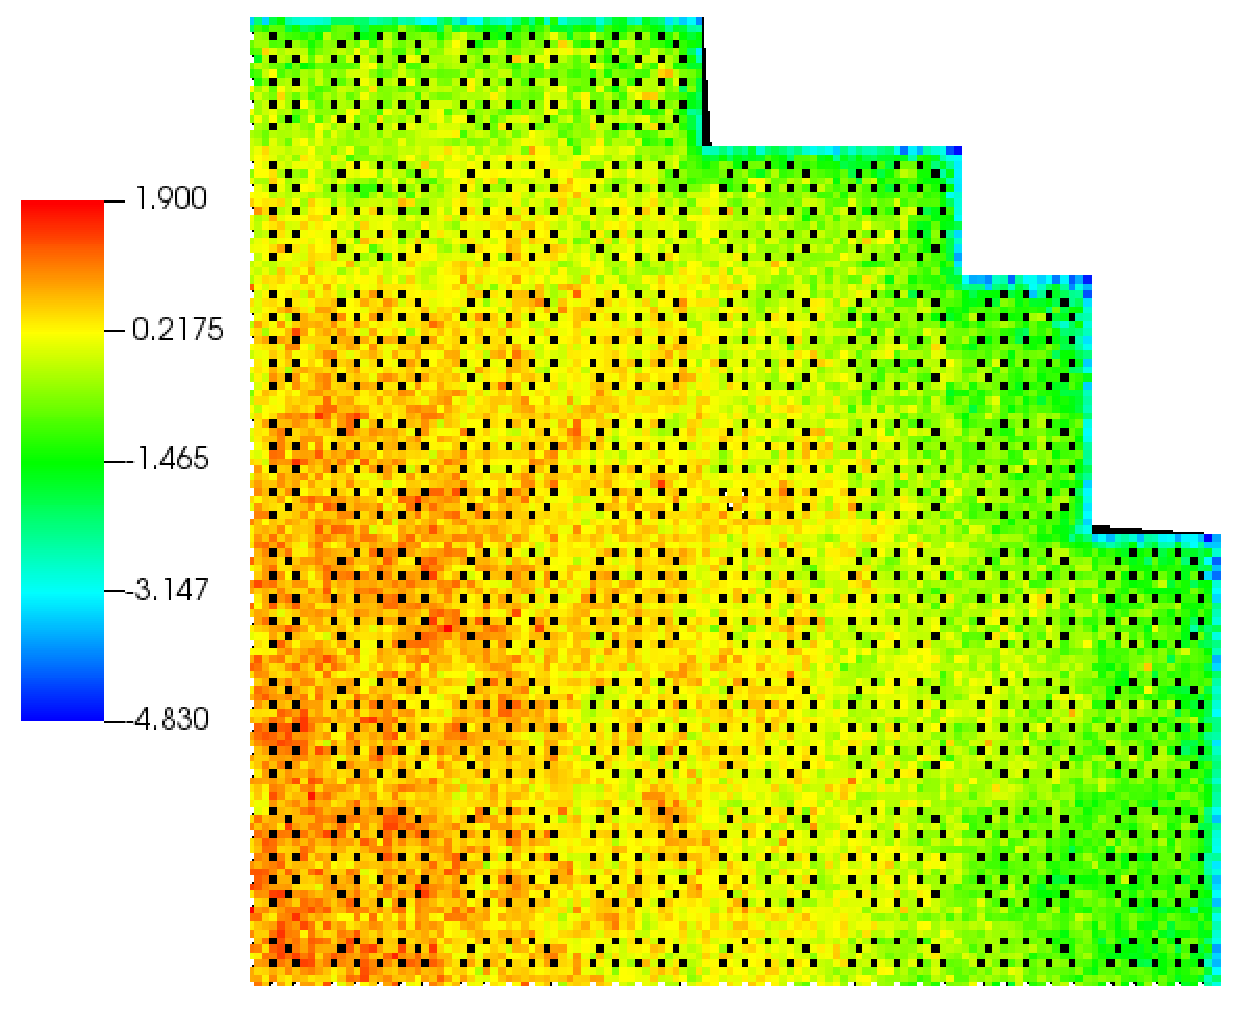
\includegraphics[width=\textwidth]{figs/pin_error_no_exp.pdf}
        \caption{No TE case}
    \end{subfigure}
    \begin{subfigure}[b]{0.5\textwidth}
        \centering
        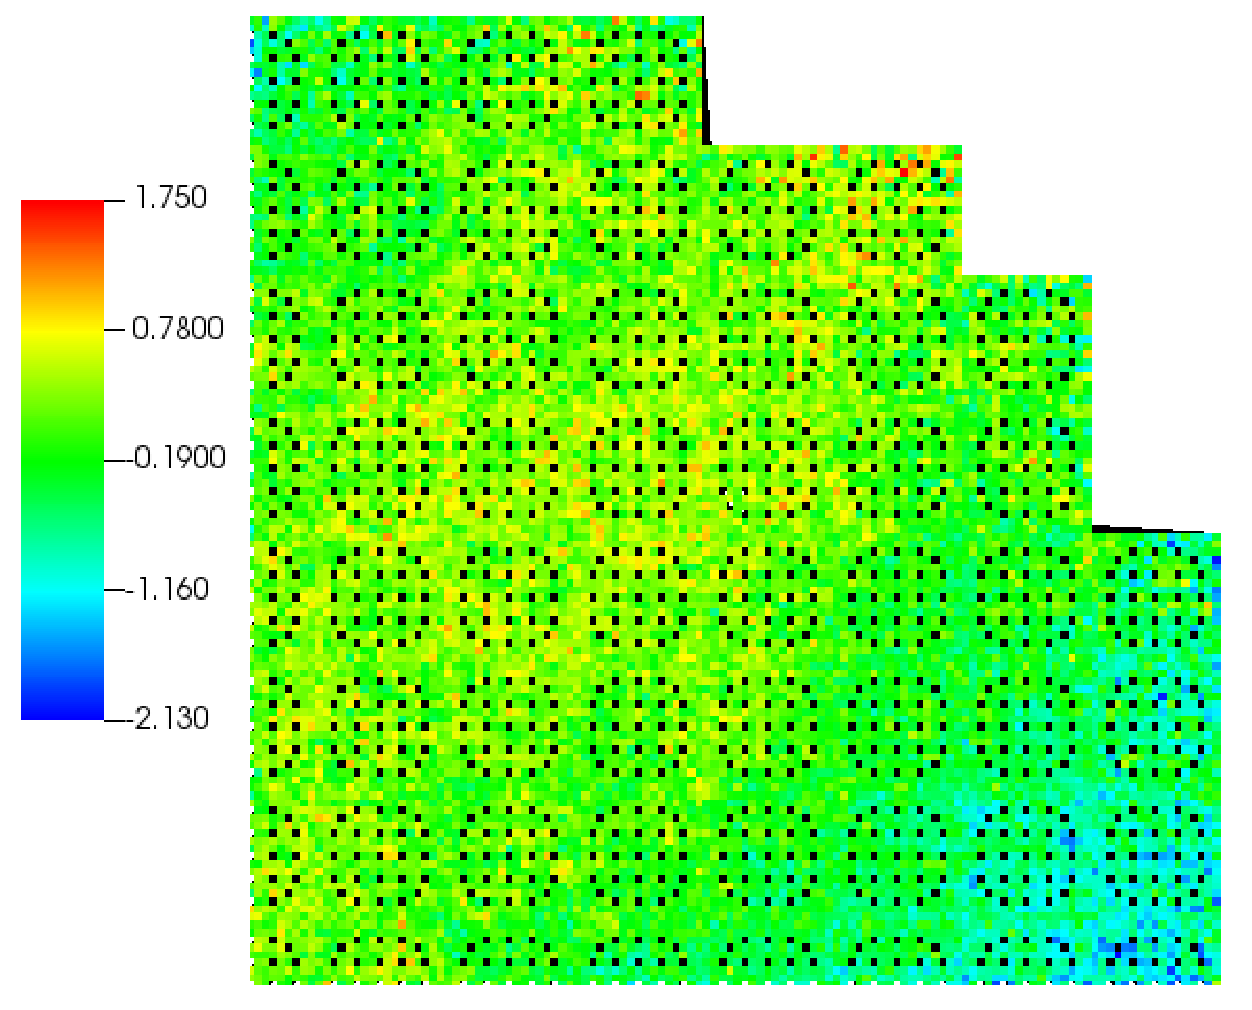
\includegraphics[width=\textwidth]{figs/pin_error_nominal.pdf}
        \caption{Core-averaged case}
    \end{subfigure}
    \begin{subfigure}[b]{0.5\textwidth}
        \centering
        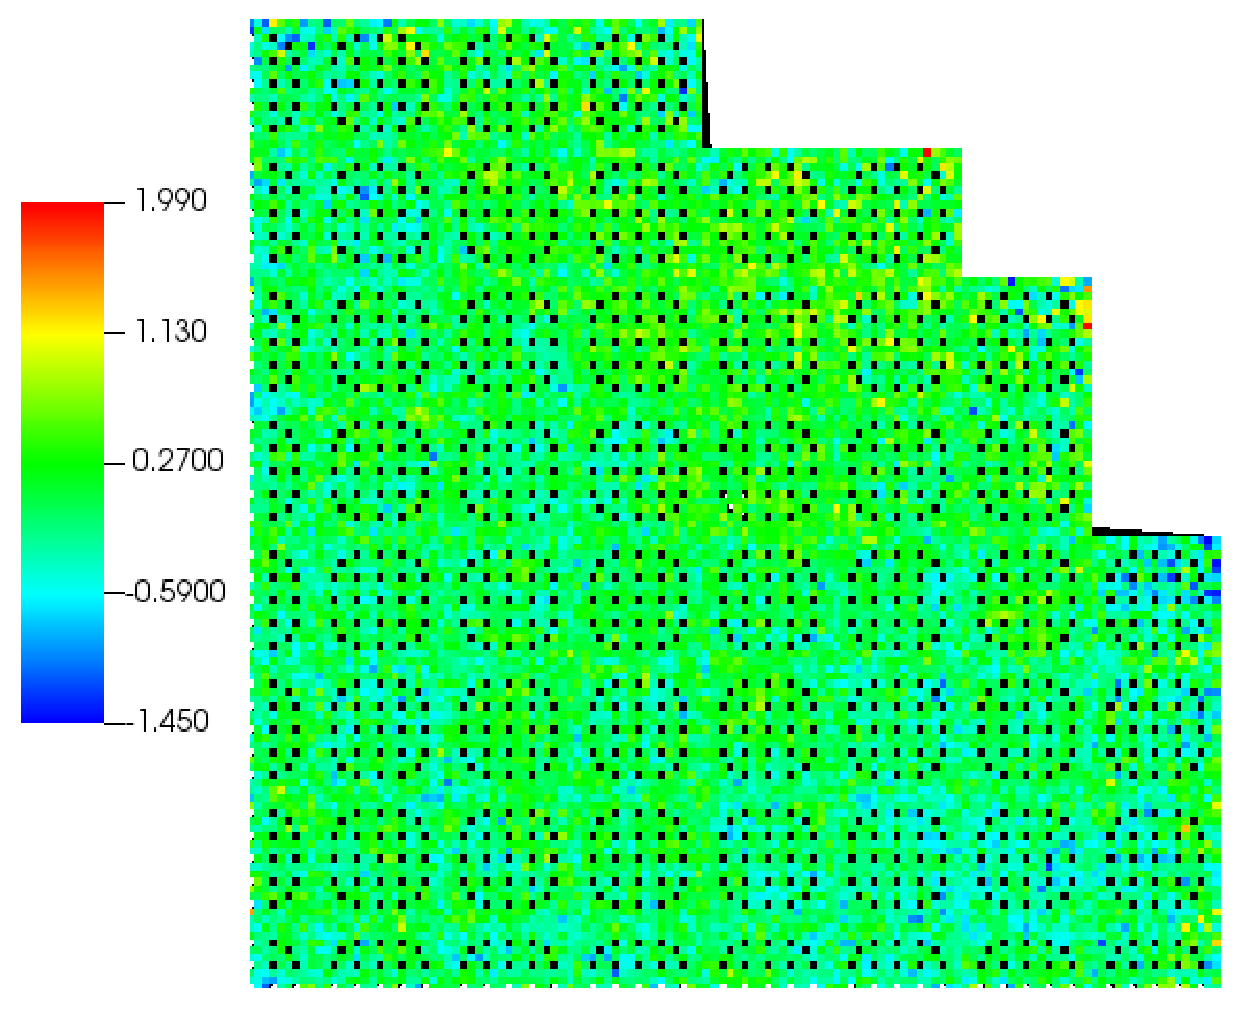
\includegraphics[width=\textwidth]{figs/pin_error_assembly.pdf}
        \caption{Assembly-averaged case}
    \end{subfigure}
    \caption[Radial pin-power errors distributions relative to the pin-averaged case]{Radial pin-power errors distributions relative to the pin-averaged for each case}
    \label{fig_421}
\end{figure}

Figure \ref{fig_421} presents the radial pin-power errors relative to the pin-averaged case. The no-TE case underestimates pin powers at the core periphery by up to -4.8\%, while overestimating pin powers near the core center. The core-averaged case yields reasonably accurate pin powers but still exhibits some deviations. The assembly-averaged case produces pin-power solutions that closely align with the pin-averaged case. Additionally, it is notable that the pin-wise case's runtime is only 0.9\% longer than the no-TE case, indicating that incorporating on-the-fly thermal expansion introduces virtually no additional computational cost.

\subsubsection{Isothermal Temperature Coefficient}

This test problems attempts to quantify the effect of thermal expansion on the isothermal temperature coefficient (ITC). The ITC represents the change in reactivity per unit change in fuel and moderator temperature \cite{ansi}. ITC measurements are typically performed during Hot Zero Power (HZP) reactor physics tests to determine whether the measured ITC aligns with the calculated value \cite{hong}.

In this study, the ITC measurement in the VERA benchmark was modeled for cases with and without TE. The reactor used in this benchmark is Watts Bar Unit 1, a Westinghouse PWR. The measured ITC was obtained during cycle 1, with all fresh fuel. The ITC was calculated using isothermal temperatures of 560 K and 570 K, with a boron concentration of 1291 ppm. 

To ensure statistical reliability, the ITC mean and the corresponding standard deviations were obtained by performing five runs for each case, with random seeds for each run. This resulted in a total of 25 ITC samples, from which the mean and standard deviation were calculated. For each run, there were 14,500 cycles, of which 2,500 cycles were inactive, with $4\times10^4$ particle histories simulated for every cycle. The results are displayed and compared against measurement result in Table \ref{tab424}.


\begin{table}
    \centering
    \caption{Calculated ITCs compared with the measured value.}
    \label{tab424} 
    % \begin{adjustbox}{width=0.6\textwidth} % Adjust your table to the text width
    \begin{tabular}{| c | c |}
    \hline 
    Cases & ITC (pcm/$^{\circ}$F) \\
     \hline
     No TE                & $-3.74 \pm 0.24 $    \\ \hline
     TE                   & $-3.31 \pm 0.22 $    \\ \hline
     Measurement          & $-2.17 $    \\ \hline
    \end{tabular}
    % \end{adjustbox}
\end{table}

As indicated in the table, incorporating TE into core modeling improves the accuracy of the ITC, bringing it closer to the measured data. Additionally, the results show that TE modeling makes the ITC more positive by 0.4 pcm/$^{\circ}$F. This difference is slightly higher than the findings in Palmtag et al. \cite{palmtag}, which reported that TE modeling increases the ITC by 0.2-0.3 pcm/$^{\circ}$F.

Although the ITC solutions for both the TE and No TE cases deviate significantly from the reported measured value, they are still comparable to the results of other MC calculations. For example, the ITC solution from KENO without TE is 3.18 pcm/$^{\circ}$F \cite{godfrey}.

\subsubsection{Whole-core Reactor Depletion using Restart Calculations}

Exercise 3 of the TVA Watts Bar Unit 1 multi-physics depletion benchmark \cite{albagami} was adopted to investigate the effect of TE on the boron letdown curve during reactor depletion. Restart cases from whole-core pin-by-pin depletion without TE were run at 0, 221.1, and 392.3 effective full power days (EFPDs) for cases with and without TE. This depletion problem simulated $6\times10^4$ particles per cycles, with a total of 5,000 cycles, of which 2,500 were active cycles.

MCS, coupled with the CTF thermal-hydraulics solver \cite{salko}, was used to solve this problem. The work on MCS/CTF multi-physics coupling was done in the previous studies \cite{yu_2017}. The results were compared against the measured values obtained from reference \cite{godfrey} and are presented in Table \ref{tab_425}.

As shown in the table, direct core modeling with TE yields more accurate predictions for this depletion whole-core problem, particularly as power increases and fuel burnup progresses. At the beginning of the cycle (BOC), core modeling with TE underestimates the measured critical boron concentration (CBC) by 22 ppm, which is slightly higher than the 13-ppm underestimation observed with core modeling without TE. This higher CBC underestimation in the TE model at BOC is attributed to the high boron concentration and zero power at the start of the cycle. However, as the fuel cycle progresses and power increases, core modeling with TE offers more precise CBC solutions. For instance, at the end of the cycle (EOC), the TE model underestimates the CBC by just 3 ppm, compared to a 27-ppm underestimation by the model without TE. These results indicate that direct core modeling with TE provides more accurate solutions, particularly at full power and higher fuel burnup levels.

\begin{table}
    \centering
    \caption{Critical boron concentrations for depletion problem.}
    \label{tab_425} 
    % \begin{adjustbox}{width=\textwidth} % Adjust your table to the text width
    \begin{tabular}{| c | c | c | c | c | c | c | }
    \hline
          &       &               &              & \multicolumn{3}{|c|}{Critical Boron Concentration (ppm)}   \\
    \cline{5-7}
     Cases & EFPDs & Percent power & Bank D step & Measurement &   TE            & No TE             \\
     \hline
     BOC    & 0.0    & 0.0           & 186         & 1299        & $1277 \pm 0.8$  &  $1286 \pm 0.6$    \\ \hline
     MOC    & 221.1  & 100.0         & 222         & 530         & $485  \pm 0.9$  &  $474  \pm 0.8$    \\ \hline
     EOC    & 392.3  & 86.9          & 202         & 38          & $35   \pm 0.9$  &  $11   \pm 0.7$    \\ \hline
    \end{tabular}
    % \end{adjustbox}
\end{table}

\clearpage
% \subsection{Combined Framework} \label{sec43}
% \subsubsection{Assembly Problem}
% \subsubsection{Whole-core Reactor Problem}
%\subsubsection{Whole-core Reactor Depletion using Restart Calculations}